\subsection{Reduced Order Observer Design}

In general an observer is utilized in a control system if either one of two specific cases occurs. If certain states in the system is not measured, an observer can be utilized to estimate the unmeasured states by utilizing the system output and input. However, it is also possible to use an observer if the measured data gathered from the sensors is affected by noise. The observer can thereby use both the noisy measured states and the estimated states creating a filtered version of the noisy states. This case will however not be utilized in the prototype.

In the attitude control an reduced order observer is used. As written in ?? the attitude model has six states, the three angles of the quadcopter (roll, pitch and yaw) and the three corresponding angular velocities. By using the Vicon system, see ??, the three angles of the quadcopter is measured. Thus making it possible to estimate the angular velocities with a reduced order observer. 

\begin{figure}[H]
\includegraphics[scale=.1]{figures/Observerdiagram1}
\centering
\captionsetup{justification=centering}
\captionof{figure}{An overall block diagram of the angular controller highlighting the observer and its corresponding inputs and output.}
\label{fig:Observerdiagram1}
\end{figure}

In \autoref{fig:Observerdiagram1} a diagram illustrating the setup of the angular controller is shown. The colored lines highlights the observer and its corresponding inputs and output.

As described in ?? the system is observable. Thus making it possible to find an observer gain, $L_{obs}$, which makes \autoref{eq:observerStable} stable.

\begin{flalign}
	A_{22} + L_{obs}A_{A12}
		\label{eq:observerStable}
\end{flalign}

The required observer gain, $L_{obs}$ ensures that the observer, see \autoref{eq:eqobservertheorem} (source:slides4), gives a estimated state, $\hat{x}_2$, which converges to $x_2$.

\begin{flalign}
	\hat{\dot{x}}_2 &= A_{21}y + A_{22}\hat{x}_2 + B_2u + L_{obs}(A_{12}\hat{x}_2 - A_{21}x_2)
		\label{eq:eqobservertheorem}
\end{flalign}

The rate in which the estimated state, $\hat{x}_2$, converges to the actual state, $x_2$, is given by the eigenvalues of \autoref{eq:observerStable}.

The observer gain, if it is large the system reacts faster, if low slower. If High you rely alot on you're sensor, since we would also increase the noise in estimator. A low gain you do not trust your sensor.

Final L matrix

Hvordan vores model vil se ud i observeren og den bliver brugt til at simulere. 

\begin{figure}[H]
	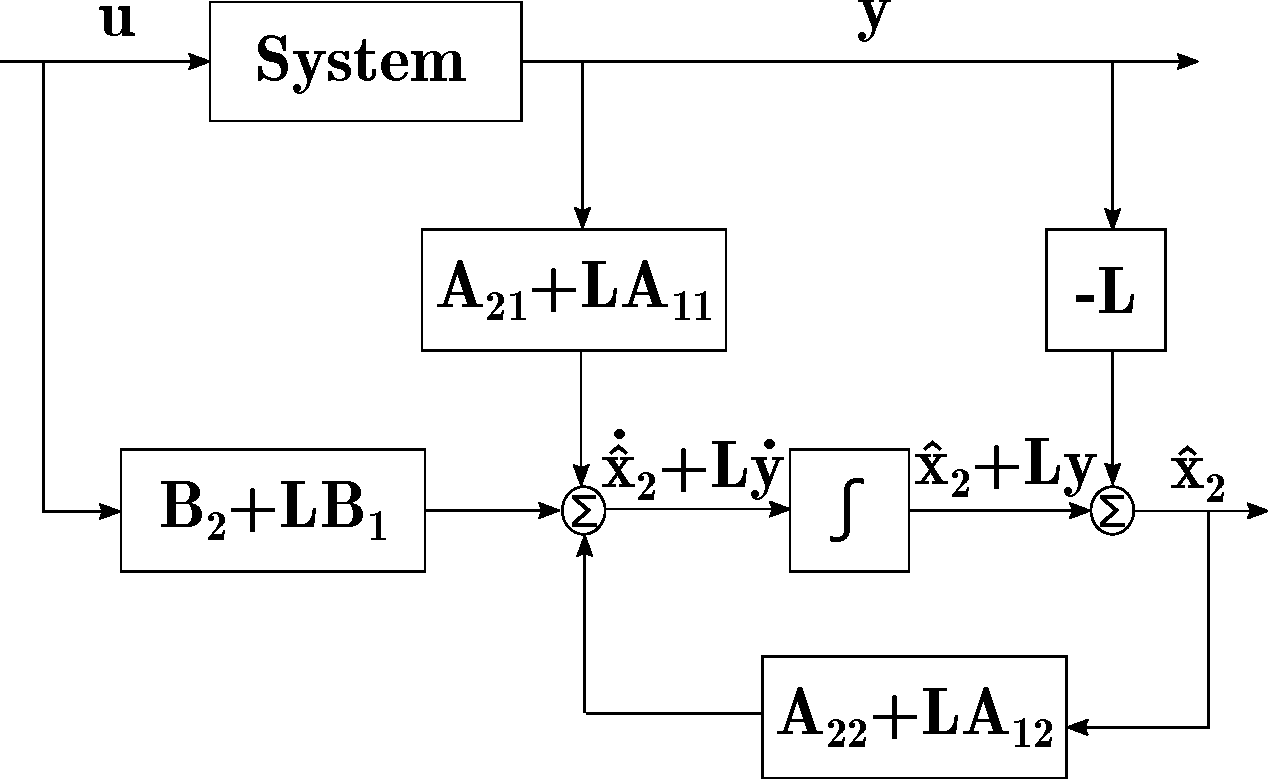
\includegraphics[scale=.35]{figures/observerDiagram}
	\centering
	\captionsetup{justification=centering}
	\captionof{figure}{Diagram . }
	\label{fig:observerDiagram}
\end{figure}

 In \autoref{fig:observerDiagram} the observer in \autoref{fig:Observerdiagram1} is opened up to illustrate how the observer is designed. BLABLABLABALA. From \autoref{fig:observerDiagram} the following \autoref{eq:eqobserverderived} is derived. 

implemented in diskrete form on the microcontroller.

\begin{flalign}
	\hat{\dot{x}}_2 + L\dot{y} &= (A_{22} + LA_{12})\hat{x}_2 + (A_{21} + LA_{11})y + (B_2 + LB_1)u
	\label{eq:eqobserverderived}
\end{flalign}









%\begin{minipage}{0.15\linewidth}
%	\begin{flalign}
%	A_{11} = 
%	\begin{bmatrix}
%		\ 0 & 0 & 0 \ \ \\ 
%		\ 0 & 0 & 0 \ \ \\ 
%		\ 0 & 0 & 0 \ \ \\
%	\end{bmatrix}	\nonumber
%	\label{A11}
%	\end{flalign}  
%\end{minipage}\hfill
%\begin{minipage}{0.15\linewidth}
%	\begin{flalign}
%	A_{12} = 
%	\begin{bmatrix}
%		\ 1 & 0 & 0 \ \ \\ 
%		\ 0 & 1 & 0 \ \ \\ 
%		\ 0 & 0 & 1 \ \ \\
%	\end{bmatrix}	\nonumber
%	\label{A12}
%	\end{flalign}
%\end{minipage}\hfill
%\begin{minipage}{0.15\linewidth}
%	\begin{flalign}
%	A_{21} = 
%	\begin{bmatrix}
%		\ 0 & 0 & 0 \ \ \\ 
%		\ 0 & 0 & 0 \ \ \\ 
%		\ 0 & 0 & 0 \ \ \\
%	\end{bmatrix}	\nonumber
%	\label{A21}
%	\end{flalign}
%\end{minipage}\hfill
%\begin{minipage}{0.15\linewidth}
%	\begin{flalign}
%	A_{22} = 
%	\begin{bmatrix}
%		\ 0 & 0 & 0 & 0 \ \ \\ 
%		\ 0 & 0 & 0 & 0 \ \ \\ 
%		\ 0 & 0 & 0 & 0 \ \ \\
%	\end{bmatrix} \nonumber
%	\label{A22}
%	\end{flalign}
%\end{minipage}\hfill
%
%
%\begin{minipage}{0.4\linewidth}
%	\begin{flalign}
%	B_1 = 
%	\begin{bmatrix}
%		\ 0 & 0 & 0 & 0 \ \ \\ 
%		\ 0 & 0 & 0 & 0 \ \ \\ 
%		\ 0 & 0 & 0 & 0 \ \ \\
%	\end{bmatrix}	\nonumber
%	\label{B1}
%	\end{flalign}
%\end{minipage}\hfill
%\begin{minipage}{0.6\linewidth}
%	\begin{flalign}
%	B_2 = 
%	\begin{bmatrix}
%		0 & \si{-\frac{2 \cdot k_{th} \cdot L \cdot \overline{\omega}_2}{J_x}} & 0 & \si{\frac{2 \cdot k_{th} \cdot L \cdot \overline{\omega}_4}{J_x}} \ \ \ \\ 
%		\ \si{\frac{2 \cdot k_{th} \cdot L \cdot \overline{\omega}_1}{J_y}} & 0 & \si{-\frac{2 \cdot k_{th} \cdot L \cdot \overline{\omega}_3}{J_y}} & 0 \ \ \ \\ 
%		\frac{2 \cdot k_d \cdot {\overline{\omega}_1}}{J_z} & - \frac{2 \cdot k_d \cdot {\overline{\omega}_2}}{J_z} & \frac{2 \cdot k_d \cdot {\overline{\omega}_3}}{J_z} & - \frac{2 \cdot k_d \cdot {\overline{\omega}_4}}{J_z} \ \ \
%	\end{bmatrix} \nonumber
%	\label{B2}
%	\end{flalign}
%\end{minipage}\hfill
%
%
%\begin{flalign}
%	L_{obs} = 
%	\begin{bmatrix}
%	\ -50 & 0 & 0  \ \ \ \\ 
%	\ 0 & -60 & 0  \ \ \ \\ 
%	\ 0 & 0 & -70  \ \ \  
%	\end{bmatrix}
%	\label{Lobs}
%\end{flalign}


